\documentclass[10pt,twocolumn]{article}
\usepackage[margin=0.75in]{geometry}
\usepackage{booktabs}
\usepackage{hyperref}
\usepackage{enumitem}
\usepackage{titlesec}
\usepackage{microtype}
\usepackage{parskip}
\usepackage{graphicx}
\usepackage{amsmath}
\usepackage{tikz}
\usepackage{pgfplots}
\pgfplotsset{compat=1.18}

\titlespacing{\section}{0pt}{6pt}{3pt}
\titlespacing{\subsection}{0pt}{4pt}{2pt}
\setlength{\columnsep}{18pt}

\title{\textbf{CSE/DSC 234 Project 2: Schema Linking with SFT}\\
\large Team 141 $\cdot$ Spring 2026}
\date{}
\author{Vincent McCloskey}

\begin{document}
\maketitle
\thispagestyle{empty}

%% ---------------------------------------------------------------
\section{Training Data Methodology}

\subsection*{Base Dataset}
The released training split contains 301 labeled NL question / schema-link pairs across 17 databases.
The distribution is highly uneven: biodiversity and government databases (NTSB, NYSED, ATBI, etc.)
each have 20--60 examples, while each of the 9 SAP Business One sub-modules has only $\sim$6.

\subsection*{Schema Serialization}
Each training prompt serializes the database schema as a list of tables and columns:
\begin{verbatim}
Table: INJURY
  [linked to: GV, OCC]
  - AIS [int,PK]
  - REGION [int]
  ...
\end{verbatim}
Three design choices drove the final format:
\begin{itemize}[noitemsep,topsep=2pt]
  \item \textit{FK links}: Each table shows which other tables it is FK-connected to, helping the model reason about joins.
  \item \textit{camelCase splitting}: Table and column names are scored against question tokens after splitting camelCase identifiers (e.g., \texttt{ExtOnErr} $\to$ \{ext, on, err\}), so relevance-based table ordering works for SAP.
  \item \textit{Relevance sorting}: Tables are ordered by how well their column names overlap with the question's tokens, placing the most likely tables before context-window truncation.
\end{itemize}
Output format is a JSON object mapping table names to column lists, using the schema's original casing.
Columns within each table are \textit{not} sorted (alphabetical sorting hurt in ablation, score $-0.04$).

\subsection*{Data Augmentation}
I wrote 105 hand-authored synthetic NL question / schema-link pairs targeting the most under-represented databases:
\begin{itemize}[noitemsep,topsep=2pt]
  \item 59 examples for all 9 SAP Business One modules (verified against schemas: 0 bad tables/columns)
  \item 46 examples for NTSB, targeting the 14 specific tables the model confused most (GV, CDC, AVOID, ADAPT, EDREVENT, ICS, OCC, VPICDECODE, CRASH)
\end{itemize}
All examples were validated programmatically against the schema JSON before training.
The combined training set is 406 examples (301 original + 105 synthetic).

\subsection*{Post-processing}
\begin{itemize}[noitemsep,topsep=2pt]
  \item \textit{Validate and drop}: All predicted table/column identifiers are checked against the schema; hallucinated ones are silently dropped.
  \item \textit{Casing correction}: Lookups are case-insensitive; output restores original schema casing.
  \item \textit{Keyword fallback}: If the model outputs empty JSON, a keyword-matching fallback predicts the most likely table based on question-token overlap with table/column names.
\end{itemize}
The fallback recovered 13 otherwise-empty predictions. Although its per-prediction accuracy is only $\sim$8\%, removing it reduces the leaderboard score (empty predictions score 0 on recall).

%% ---------------------------------------------------------------
\section{Final Pipeline Architecture}

\subsection*{Base Model}
\texttt{Qwen/Qwen2.5-1.5B-Instruct} (1.5B parameters). Selected over Qwen3-1.7B (single-stage inference took 11.3\,min, borderline for the 15-min budget) and Qwen2.5-0.5B (weaker structured-output discipline on large schemas).

\subsection*{LoRA Adapter}
\begin{itemize}[noitemsep,topsep=2pt]
  \item Rank $r=32$, $\alpha=64$, dropout 0.05
  \item Target modules: \texttt{q\_proj, k\_proj, v\_proj, o\_proj}
  \item Training: 6 epochs, lr = $8 \times 10^{-5}$, cosine schedule, batch 1, grad accum 16 (effective batch 16)
  \item Max sequence length: 2048 tokens
  \item Trained on NVIDIA L4 (23\,GB), $\sim$30\,min
\end{itemize}
The adapter is committed at \texttt{adapter/} ($\sim$34\,MB).

\subsection*{Prompt Template}
\begin{verbatim}
System: You are a schema linking assistant.
  Given a question and schema, output a JSON
  object mapping each referenced table to a
  list of referenced column names. Use [] for
  tables referenced without specific columns
  (e.g. COUNT(*)). Output only valid JSON.

User:
Database: {db_id}
Schema:
{serialized_schema}

Question: {question}
\end{verbatim}

\subsection*{Two-Stage Inference}
Stage\,1 (full-schema prediction) runs the model on the truncated schema to predict tables and columns.
Stage\,2 (column refinement) runs a second, focused pass for each predicted table:
\begin{verbatim}
System: You are a column linking assistant.
  Given a question and one table with its
  columns, output a JSON array of referenced
  column names, or [] if none.

User:
Question: {question}
Table: {table}
Columns:
  - Col1 [type]
  - Col2 [type,PK]
  ...
\end{verbatim}
Stage\,2 improved column score from 0.339 to 0.394 (+16\%) by giving the model isolated, focused context per table rather than asking it to track column attribution across 40+ tables simultaneously.
Inference time on the grading pod: \textbf{3.2\,min} for 101 questions (well within the 15-min budget).

\subsection*{Schema Truncation}
For large schemas (SAP Finance has 61 tables, NTSB has 40 tables with 1161 columns), the prompt exceeds 6000 tokens. We truncate the schema body from the bottom (removing less-relevant tables), preserving the system prompt and the question. A binary search over line count finds the maximum schema that fits within 2360 tokens (3072 $-$ 512 generation reserve $-$ 200 overhead), ensuring the model always sees the question.

%% ---------------------------------------------------------------
\section{Experimentation Methodology}

I ran 30+ distinct configurations over three phases: (1) RapidFire AI multi-config grid for initial exploration, (2) \texttt{train\_simple.py} single-config runs for fine-grained control, and (3) inference-time ablations on the best adapter.

\textbf{RapidFire AI experiments} (\texttt{schema-linking-v1} through \texttt{v4}): 2 base models (Qwen2.5-0.5B, 1.5B) $\times$ 2 LoRA ranks ($r \in \{8, 32\}$) $\times$ 2 learning rates ($\{2\times10^{-4}, 5\times10^{-5}\}$) = 8 configs per experiment. These established that 1.5B outperforms 0.5B and larger rank helps.

\textbf{Key knobs varied:}

\vspace{4pt}
\noindent\textbf{Table 1: Config knob summary}
\vspace{2pt}

\begin{center}
\scriptsize
\setlength{\tabcolsep}{3pt}
\begin{tabular}{@{}llr@{}}
\toprule
Knob & Values tested & Winner \\
\midrule
Base model & 0.5B, 1.5B, Qwen3-1.7B & 1.5B \\
LoRA rank & 8, 16, 32, 64 & 32 \\
Learning rate & 1e-4, 8e-5, 6e-5, 5e-5 & 8e-5 \\
Epochs & 3, 5, 6, 7, 8, 10 & 6 \\
Schema: FK links & on, off & on \\
Schema: table sort & on, off & on \\
Schema: camelCase split & on, off & on \\
Schema: table descriptions & on (hardcoded), off & off \\
Schema: sorted output & on, off & off \\
Inference: two-stage & on, off & on \\
Inference: topk fallback & 0, 2, 3 & 0 \\
Stage2: multi-table ctx & on, off & off \\
Synthetic data (SAP) & 0, 39, 59, 67 examples & 59 clean \\
Synthetic data (NTSB) & 0, 46 examples & 46 \\
Oversample factor & 1, 2, 3, 4 & 1 \\
\bottomrule
\end{tabular}
\end{center}

%% ---------------------------------------------------------------
\section{Results and Analysis}

\subsection*{Score Progression}

\vspace{4pt}
\noindent\textbf{Table 2: Key milestones}
\vspace{2pt}

\begin{center}
\small
\begin{tabular}{@{}lcc@{}}
\toprule
Configuration & Table & Overall \\
\midrule
Baseline (5ep, 1024 tok) & 0.246 & 0.206 \\
+ keyword fallback & 0.246 & 0.313 \\
+ FK links in schema & 0.363 & 0.334 \\
+ table sorting & 0.389 & 0.354 \\
+ left-truncation fix & 0.459 & 0.398 \\
+ synthetic SAP (39 ex) & 0.495 & 0.425 \\
+ camelCase split (ablation) & 0.499 & 0.419 \\
+ two-stage inference & 0.499 & \textbf{0.440} \\
+ $r=32$, lr=$8\times10^{-5}$ & 0.517 & \textbf{0.454} \\
+ synthetic NTSB (46 ex) & 0.499 & 0.454 \\
\bottomrule
\end{tabular}
\end{center}

\begin{figure}[h]
\centering
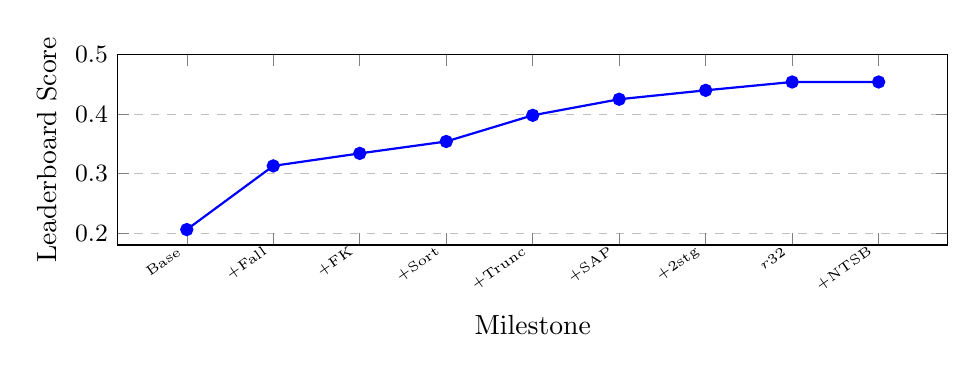
\begin{tikzpicture}
\begin{axis}[
  width=\columnwidth, height=4cm,
  xlabel={Milestone}, ylabel={Leaderboard Score},
  xtick={1,2,3,4,5,6,7,8,9},
  xticklabels={Base,+Fall,+FK,+Sort,+Trunc,+SAP,+2stg,$r$32,+NTSB},
  xticklabel style={font=\tiny, rotate=35, anchor=east},
  ymin=0.18, ymax=0.50,
  ymajorgrids=true, grid style=dashed,
  tick label style={font=\small},
]
\addplot[mark=*, thick, color=blue] coordinates {
  (1,0.206)(2,0.313)(3,0.334)(4,0.354)(5,0.398)(6,0.425)(7,0.440)(8,0.454)(9,0.454)
};
\end{axis}
\end{tikzpicture}
\caption{Leaderboard score progression across major milestones.}
\end{figure}

\subsection*{What Worked}

\textbf{Two-stage inference (+0.021)} was the largest single inference-time gain. Stage\,1 predicts tables but often gets columns wrong (72/101 predictions had at least one wrong column before stage\,2). Giving the model a focused, single-table context for column prediction improved precision from 0.35 to 0.42. The key insight: with 40+ tables visible, the model loses track of which columns belong to which table; with one table in context, it cannot make attribution errors.

\textbf{Larger LoRA rank $r=32$ (+0.015)} gave meaningful capacity gains over $r=16$. The model needs to memorize associations between cryptic table abbreviations (GV, CDC, AVOID) and natural-language concepts; $r=64$ overfit, $r=32$ was the sweet spot.

\textbf{Lower learning rate ($8\times10^{-5}$) over fewer epochs (+0.015)} outperformed faster training ($1\times10^{-4}$, 5 epochs) and slower training ($5\times10^{-5}$, 8 epochs). More epochs consistently overfit on this small dataset (301--406 examples).

\textbf{FK links in schema (+0.021)} helped because the model can reason about joins from the structural hints, even for tables it hasn't seen in training.

\textbf{Fixing truncation direction (+0.044)} was the biggest single bug fix. The original code truncated from the left (cutting the system prompt), causing the model to see only schema text and output garbled schema continuations instead of JSON. Switching to truncate the schema body from the bottom (preserving the system prompt and question) immediately fixed the empty-prediction problem.

\textbf{Synthetic SAP data (+0.027)} doubled SAP coverage from $\sim$6 to $\sim$13 examples per module, directly improving the six SAP databases that were stuck at 0.000.

\subsection*{What Did Not Work}

\textbf{Hardcoded table descriptions} (e.g., ``GV [General Vehicle info: make, model, year, lighting condition]'') scored 0.4446 when trained and inferred with descriptions vs.\ 0.4539 without. The descriptions add tokens that push relevant table columns past the truncation boundary.

\textbf{Qwen3-1.7B} scored 0.4356 single-stage and required 11.3\,min inference vs.\ 3.2\,min for Qwen2.5-1.5B with two-stage. The newer architecture did not outperform the tuned 1.5B model.

\textbf{FK propagation} (adding FK-connected tables with column overlap as post-processing) scored 0.4177 vs.\ 0.4539: adding extra tables lowered precision more than it helped recall.

\textbf{Column sorting in output} scored 0.4058 vs.\ 0.4539: alphabetical ordering destabilized the decoding distribution.

\subsection*{Failure Analysis}

A diagnostic breakdown of 101 validation predictions reveals three failure modes:
\begin{itemize}[noitemsep,topsep=2pt]
  \item \textit{Completely wrong table} (35 questions, 35\%): model predicts a plausible but incorrect table. NTSB accounts for 14 of these --- the model defaults to high-frequency training tables (AIRBAG, CHILDSEAT) regardless of question content.
  \item \textit{Partial table set} (28 questions, 28\%): model gets some but not all tables for multi-table join queries.
  \item \textit{Correct tables, wrong columns} (3 questions): table prediction is correct but column attribution fails.
\end{itemize}
The 35 wrong-table failures are a pure model limitation, not a pipeline bug. There are no casing mismatches, no JSON parse failures, and no empty predictions. The model simply cannot distinguish 40 cryptic NTSB table names (GV, CDC, OCC, AVOID...) with only 60 training examples.

\subsection*{Per-Database Breakdown (final model)}

\begin{center}
\scriptsize
\begin{tabular}{@{}lcc@{}}
\toprule
Database & $n$ & Avg F1 \\
\midrule
ASIS\_20161108\_HerpInv & 8 & 0.773 \\
NorthernPlainsFireMgmt & 8 & 0.788 \\
CratersWildlife & 8 & 0.631 \\
NYSED\_SRC2022 & 13 & 0.472 \\
PacificIslandLandbirds & 8 & 0.503 \\
KlamathInvasive & 8 & 0.393 \\
ATBI & 8 & 0.369 \\
NTSB & 20 & 0.205 \\
SAP databases (9) & 20 & 0.00--0.35 \\
\bottomrule
\end{tabular}
\end{center}

\subsection*{With More Time}
The two highest-leverage remaining improvements would be: (1) 50+ additional NTSB training examples covering all 40 table abbreviations with human-readable descriptions baked into the training schema (not inference), so the model learns the association at training time; and (2) a retrieval-augmented fallback that, for databases the model is uncertain on, looks up similar training examples at inference time to provide in-context demonstrations.

%% ---------------------------------------------------------------
\section{AI Tools Statement}

Claude Code (\texttt{claude-sonnet-4-6} 1M context) was used for partial code generation and to simplify running commands over SSH on the DSMLP compute cluster. All experimental design decisions, hyperparameter choices, data curation, and interpretations of results were made by the author.

\end{document}
